% Options for packages loaded elsewhere
\PassOptionsToPackage{unicode}{hyperref}
\PassOptionsToPackage{hyphens}{url}
%
\documentclass[
]{article}
\usepackage{amsmath,amssymb}
\usepackage{iftex}
\ifPDFTeX
  \usepackage[T1]{fontenc}
  \usepackage[utf8]{inputenc}
  \usepackage{textcomp} % provide euro and other symbols
\else % if luatex or xetex
  \usepackage{unicode-math} % this also loads fontspec
  \defaultfontfeatures{Scale=MatchLowercase}
  \defaultfontfeatures[\rmfamily]{Ligatures=TeX,Scale=1}
\fi
\usepackage{lmodern}
\ifPDFTeX\else
  % xetex/luatex font selection
\fi
% Use upquote if available, for straight quotes in verbatim environments
\IfFileExists{upquote.sty}{\usepackage{upquote}}{}
\IfFileExists{microtype.sty}{% use microtype if available
  \usepackage[]{microtype}
  \UseMicrotypeSet[protrusion]{basicmath} % disable protrusion for tt fonts
}{}
\makeatletter
\@ifundefined{KOMAClassName}{% if non-KOMA class
  \IfFileExists{parskip.sty}{%
    \usepackage{parskip}
  }{% else
    \setlength{\parindent}{0pt}
    \setlength{\parskip}{6pt plus 2pt minus 1pt}}
}{% if KOMA class
  \KOMAoptions{parskip=half}}
\makeatother
\usepackage{xcolor}
\usepackage{graphicx}
\makeatletter
\def\maxwidth{\ifdim\Gin@nat@width>\linewidth\linewidth\else\Gin@nat@width\fi}
\def\maxheight{\ifdim\Gin@nat@height>\textheight\textheight\else\Gin@nat@height\fi}
\makeatother
% Scale images if necessary, so that they will not overflow the page
% margins by default, and it is still possible to overwrite the defaults
% using explicit options in \includegraphics[width, height, ...]{}
\setkeys{Gin}{width=\maxwidth,height=\maxheight,keepaspectratio}
% Set default figure placement to htbp
\makeatletter
\def\fps@figure{htbp}
\makeatother
\setlength{\emergencystretch}{3em} % prevent overfull lines
\providecommand{\tightlist}{%
  \setlength{\itemsep}{0pt}\setlength{\parskip}{0pt}}
\setcounter{secnumdepth}{-\maxdimen} % remove section numbering
\ifLuaTeX
  \usepackage{selnolig}  % disable illegal ligatures
\fi
\IfFileExists{bookmark.sty}{\usepackage{bookmark}}{\usepackage{hyperref}}
\IfFileExists{xurl.sty}{\usepackage{xurl}}{} % add URL line breaks if available
\urlstyle{same}
\hypersetup{
  hidelinks,
  pdfcreator={LaTeX via pandoc}}

\author{}
\date{}

\begin{document}

\textbf{Imperial College London}

\textbf{Department of Earth Science and Engineering}

\textbf{MSc Environmental Data Science and Machine Learning}

\textbf{Project plan:}

\textbf{Predicting Individual Physiological Responses to Pollution Using
Transformer-Based Time-Series Models}

\textbf{Davide Baino}

\textbf{Email:
\href{mailto:davide.baino24@imperial.ac.uk}{\nolinkurl{davide.baino24@imperial.ac.uk}}}

\textbf{GitHub: esemsc-db24}

\textbf{Supervisor:}

\textbf{Dr. Christopher Pain}

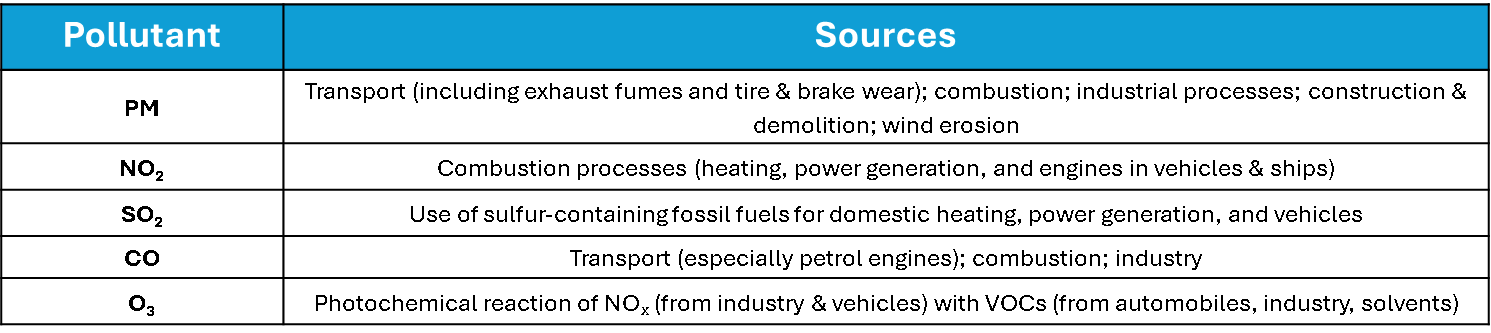
\includegraphics[width=1.77215in,height=1.8984in]{media/image1.png}

\hypertarget{table-of-contents}{%
\section{Table of Contents}\label{table-of-contents}}

\protect\hyperlink{abstract}{1. Abstract
\protect\hyperlink{abstract}{3}}

\protect\hyperlink{problem-description}{2 Problem Description
\protect\hyperlink{problem-description}{3}}

\protect\hyperlink{rationale-and-literature-review}{2.1 Rationale and
Literature Review
\protect\hyperlink{rationale-and-literature-review}{3}}

\protect\hyperlink{objectives}{2.2 Objectives
\protect\hyperlink{objectives}{4}}

\protect\hyperlink{dataset}{3 Dataset \protect\hyperlink{dataset}{4}}

\protect\hyperlink{methodology}{4 Methodology
\protect\hyperlink{methodology}{6}}

\protect\hyperlink{timeline}{5 Timeline \protect\hyperlink{timeline}{8}}

\hypertarget{abstract}{%
\section{\texorpdfstring{\hfill\break
1. Abstract}{ 1. Abstract}}\label{abstract}}

Air pollution remains a major global health and environmental concern,
contributing to an estimated seven million deaths annually through the
combined effects of outdoor and household exposure
(\href{https://www.who.int/health-topics/air-pollution\#tab=tab_2}{WHO,}
2025){[}1{]}. While pollution levels are projected to decline, the
ongoing impacts of climate change continue to pose serious risks.
Simultaneously, advancements in wearable sensor technologies allow for
the systematic collection of high-resolution physiological data over
long periods of time (Roos \& Slavich, 2023){[}2{]}.

This study aims to develop an identity map linking varying levels of air
pollution to individual physiological responses. Such a framework will
enable the prediction of health responses to pollution exposure,
facilitating early warnings and personalised health recommendations. To
achieve this, we propose a two-model approach: an initial general model
to capture population-wide temporal trends, and a personalised one
fine-tuned to individual characteristics. Together, these models will
enhance the precision of forecasting and contribute to more effective,
data-driven health interventions when reacting to a polluted
environment.

\hypertarget{problem-description}{%
\section{\texorpdfstring{2. Problem Description
}{2. Problem Description }}\label{problem-description}}

\hypertarget{rationale-and-literature-review}{%
\subsection{2.1 Rationale and Literature
Review}\label{rationale-and-literature-review}}

Air pollution represents a critical challenge in the 21st century, with
significant implications for human health. For example, He et al.
{[}3{]} estimate that air pollution reduces average life expectancy by
1.8 years worldwide and up to 3 years in highly polluted regions of
China.

Pollution occurs when substances from human, biological, or natural
sources enter the atmosphere at concentrations beyond typical levels,
posing short- or long-term risks (Bernasconi, Angelucci, \& Aliverti,
2022){[}4{]}. Pollutants are categorized as either primary (directly
emitted, such as PM, CO, and NO) or secondary (formed through chemical
reactions, like O₃ and NO₂, often found far from their original
sources). This study primarily examines criteria
pollutants---particularly PM₁₀ and PM₂.₅---due to their severe health
risks (Bernasconi, Angelucci, \& Aliverti, 2022){[}4{]}.

Historically, air quality has been monitored using fixed-location
stations, providing aggregated environmental data at a city or regional
level. While useful for assessing general air quality trends, this
approach presents a major limitation: it overlooks personal exposure to
pollution. These static measurements fail to capture the dynamic and
highly individualised nature of pollution exposure, which varies
significantly depending on a person's location, mobility patterns, and
daily activities (Hu et al., 2014){[}5{]}. For instance, walking,
jogging, or commuting through high-traffic areas can expose individuals
to different pollution levels even within the same location (Hu et al.,
2014){[}5{]}. Moreover, the same pollutant concentration may cause
varying physiological responses across individuals, depending on factors
such as health status, age, pre-existing respiratory conditions, and
lifestyle (Hu et al., 2014){[}5{]}. As a result, population-level
estimates often obscure the true, personalised impact of air pollution
on human health (Hu et al., 2014){[}5{]}.

Recent research has improved pollution forecasting, yet gaps remain in
linking these predictions to health outcomes. For example, the Breath
study employs a transformer-based model to predict NO₂ levels in India
with high accuracy (Verma et al., 2024){[}6{]}. However, it does not
explore how these pollution fluctuations affect individual or population
health, limiting its utility for policymaking or preventative
healthcare.

In contrast, Atzeni et al. (2025){[}7{]} developed a machine learning
pipeline for short-term respiratory disease prediction. Their work
underscores the importance of stratifying individuals before modelling
and demonstrates the effectiveness of traditional methods like Logistic
Regression, Random Forest, and XGBoost. Nevertheless, it does not
leverage modern deep learning techniques for time-series analysis, which
could better capture temporal patterns in physiological data.

\hypertarget{objectives}{%
\subsection{2.2 Objectives}\label{objectives}}

The approach proposed in this study directly addresses the challenge
outlined in the BEHRT initiative by integrating IoT-enabled wearable
devices to support proactive and personalised health interventions Li,
Y. et al. (2020){[}8{]}. To this end, a transformer-based time-series
deep learning architecture is proposed. The first objective is to
harness the transformer's strength in modelling long-range temporal
dependencies to identify population-level trends, thereby enabling the
construction of an identity map that links pollution exposure to
physiological responses. The second objective is to deliver real-time,
individualised insights---alerting users to expect physiological changes
when encountering similar pollution levels in the future.

\hypertarget{dataset}{%
\section{3. Dataset}\label{dataset}}

The datasets used in this study come from two distinct sources, offering
complementary information to investigate the relationship between air
pollution and individual health responses.

The first dataset is provided by the INHALE project and consists of data
from 59 participants aged between 20 and 75 years, including 33
non-asthmatic and 26 asthmatic individuals. Each participant was
equipped with wearable sensors that recorded information on air
pollution exposure, respiratory health, and physical activity. Although
the temporal coverage of the INHALE dataset is limited, data collection
during two distinct two-week periods during summer or winter, it
provides a more targeted view of personalised exposure and associated
health outcomes over different time periods, as shown in figure 1

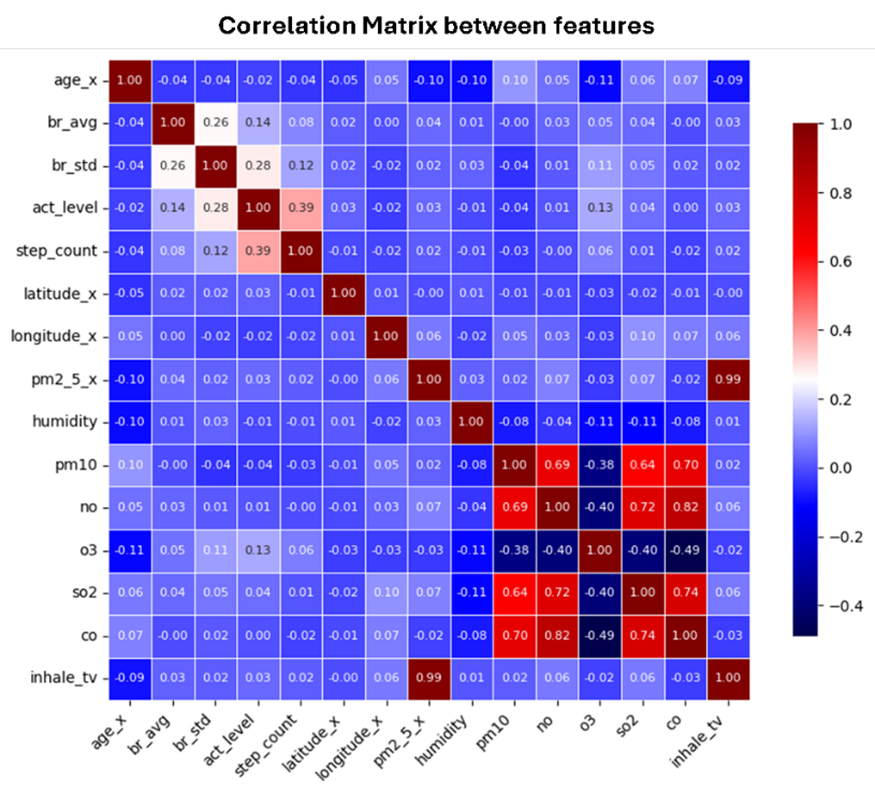
\includegraphics[width=6.26806in,height=3.13403in]{media/image2.jpeg}

\emph{Figure 1: Hourly PM₂.₅ levels from the INHALE dataset, showing
clear peaks in individual exposure between 18:00 and 21:00.}

The second dataset comes from the OpenWeather API and provides real-time
air pollution levels, including key pollutants such as PM2.5 and NO2.
Crucially, this dataset is geolocated using GPS coordinates, offering
pollution data at a spatial resolution of approximately 200 metres. When
matched with the location data collected through Inhale, this enables a
spatially-aware analysis of personal exposure to air pollution, allowing
for the integration of environmental data with individual physiological
responses. Although a 200-metre resolution may not capture highly
localised variations in pollution, this limitation is mitigated by the
more granular exposure data available directly from the INHALE dataset.

\hypertarget{methodology}{%
\section{4. Methodology}\label{methodology}}

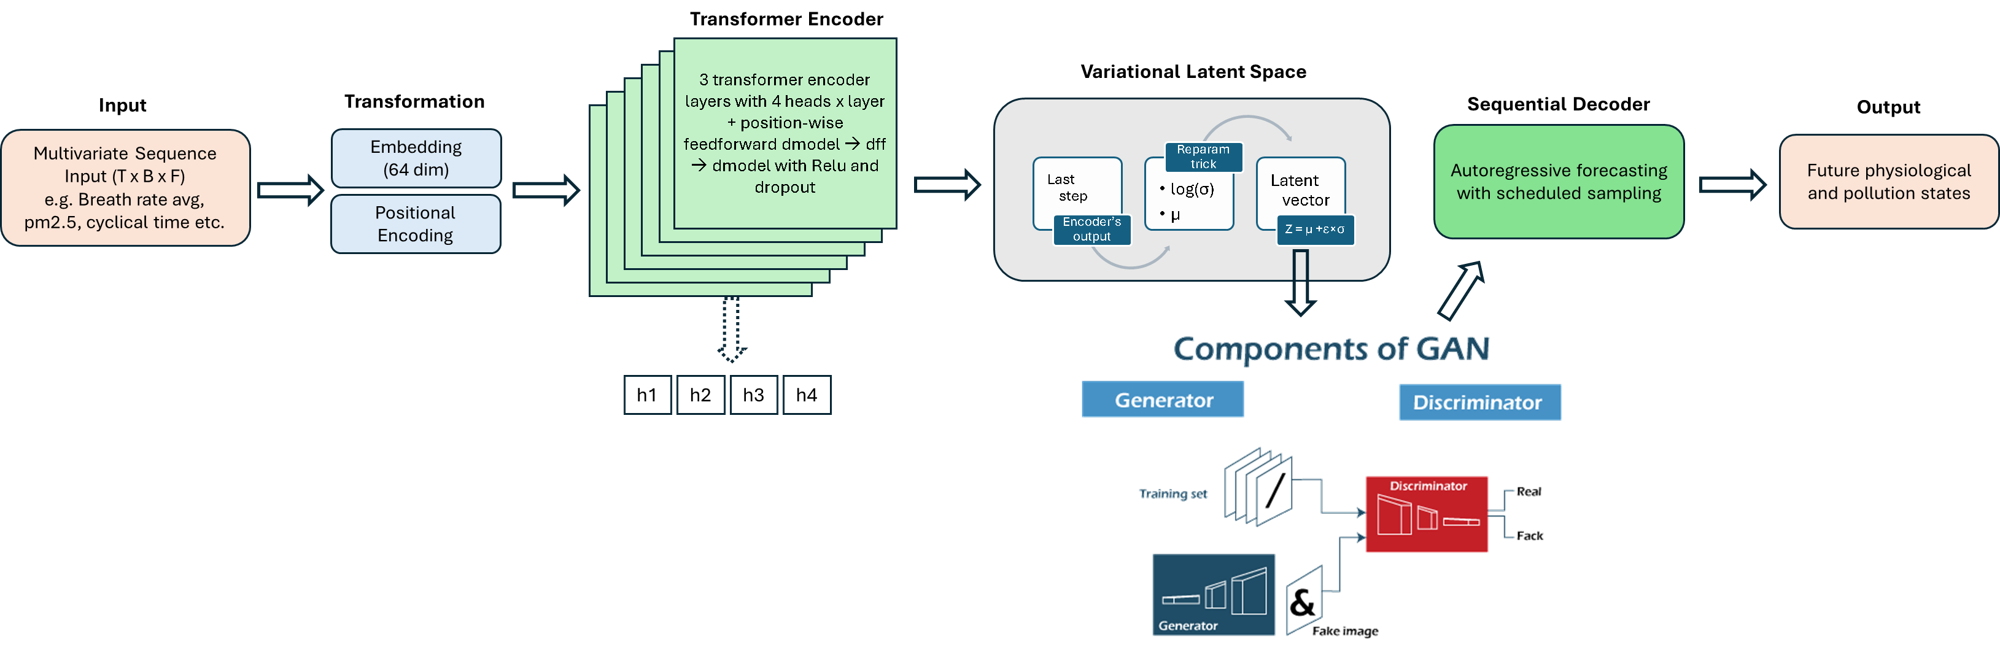
\includegraphics[width=6.47702in,height=3.72196in]{media/image3.png}

\emph{Figure 2: General transformer-based architecture, trained on
OpenWeather and INHALE architecture and subsequently fine-tuned at
individual level.}

The analysis begins with ingesting and exploring both datasets through
comprehensive exploratory data analysis (EDA) to examine feature
distributions, scales, and relationships. Given the heterogeneity of
variables---ranging from physiological metrics to pollution
indicators---normalisation will standardise scales for comparability.
Missing data will be addressed via imputation, with time-series methods
(e.g., ARIMA) applied for temporal gaps and Multiple Imputation by
Chained Equations (MICE) for statistically missing values, guided by
missingness patterns. Outliers, particularly those arising from wearable
sensor noise, will be identified and corrected to ensure data fidelity.

To interpret feature relevance, SHAP (Shapley Additive Explanations)
values will be computed to quantify the contribution of each variable to
model predictions (Lundberg \& Lee, 2017){[}9{]}. Following data
cleaning and transformation, an initial unsupervised clustering approach
(e.g., k-means) will group individuals based on their responses to
pollution exposure. This acknowledge the heterogeneity of how
individuals react to similar pollution level , as shown in figure 2.

The resulting cluster labels, representing individual classes, will be
integrated into a hybrid modelling framework. Each input sequence will
include the individual's assigned class, wearable-derived physiological
signals, and pollution variables all spatially linked through GPS
coordinates. These will be fed into a time-series transformer
architecture structured as an encoder-decoder model. The transformer
encoder will learn latent representations of long-range dependencies
across time, leveraging multi-head attention to capture complex
interactions between variables as explained in figure 3 (Vaswani et al.,
2017){[}10{]}. This latent representation will serve as an identity map,
associating pollution levels with corresponding physiological responses.
The transformer decoder will then use this representation to forecast
future states, effectively predicting the body's response to
environmental changes across a prediction horizon. To improve long-range
forecasting performance, the model will recursively uses its own
predictions as inputs for subsequent time steps, promoting robustness
and maintaining low mean squared error (MSE) over longer time spans.

Once general trends have been captured by the global model, a
fine-tuning phase will adapt the model to individual-level data. This
personalised calibration will enhance the model's ability to deliver
real-time alerts, enabling proactive intervention by predicting
individual physiological responses under anticipated pollution
conditions.

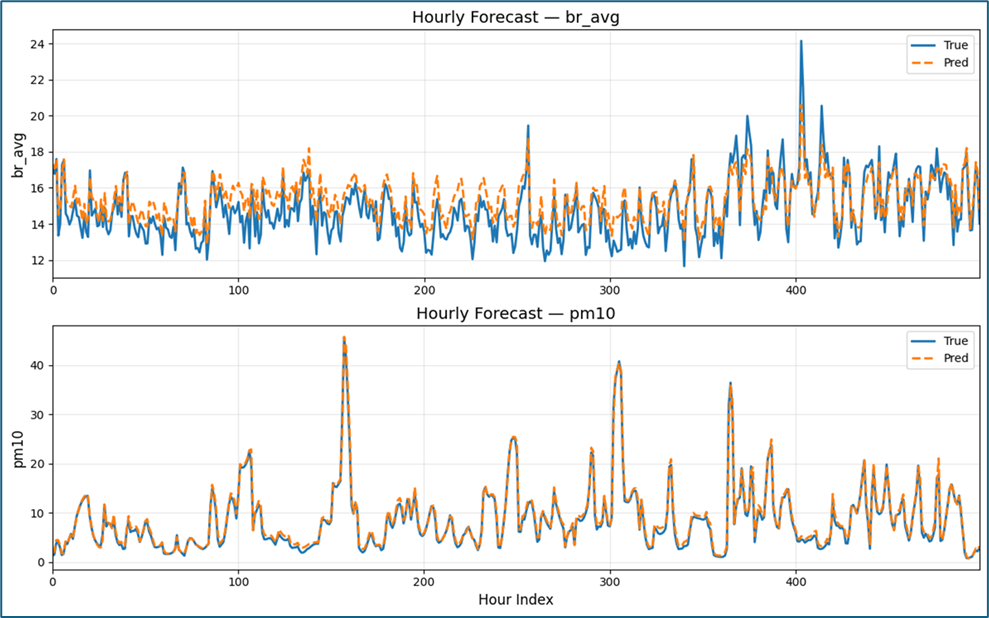
\includegraphics[width=6.26806in,height=3.34306in]{media/image4.png}

\emph{Figure 3: Time-series Transformer architecture mapping input
features to a latent space}

To evaluate the limitations of the proposed approach, we trained an
encoder--decoder Transformer on a synthetic sine‐wave time series and
assessed its ability to extrapolate 100 steps into the future. Including
encoder-decoder blocks and positional encodings was key for the model to
internalise both temporal ordering and relative distance information.
Without both the model would lack the concept of time. In practice, the
network achieves near‐zero training and test MAE on this toy task,
demonstrating its capacity to capture smooth periodic structure and
generate accurate long‐horizon forecasts. However, the model's
performance largely reflects the simplicity of the sine wave. Also,
forecast error typically amplifies with horizon length---an effect that
should be quantified by plotting step‐wise MAE growth.

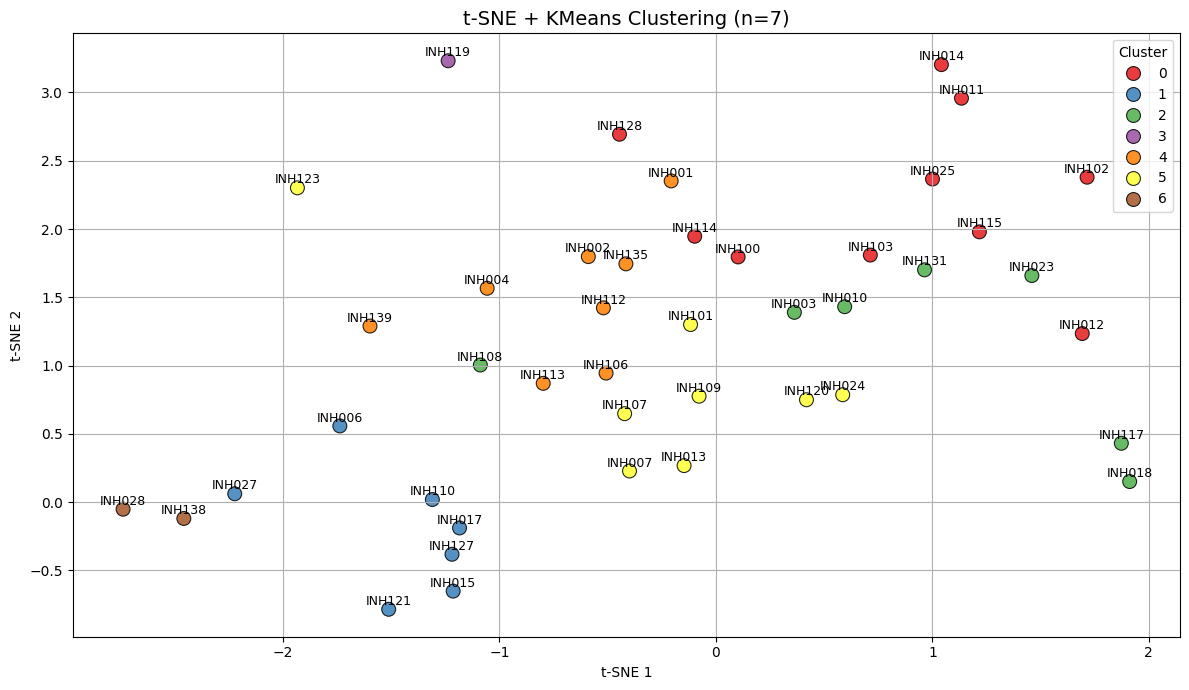
\includegraphics[width=6.26806in,height=2.87292in]{media/image5.png}

Figure 4

\hypertarget{timeline}{%
\section{5. Timeline}\label{timeline}}

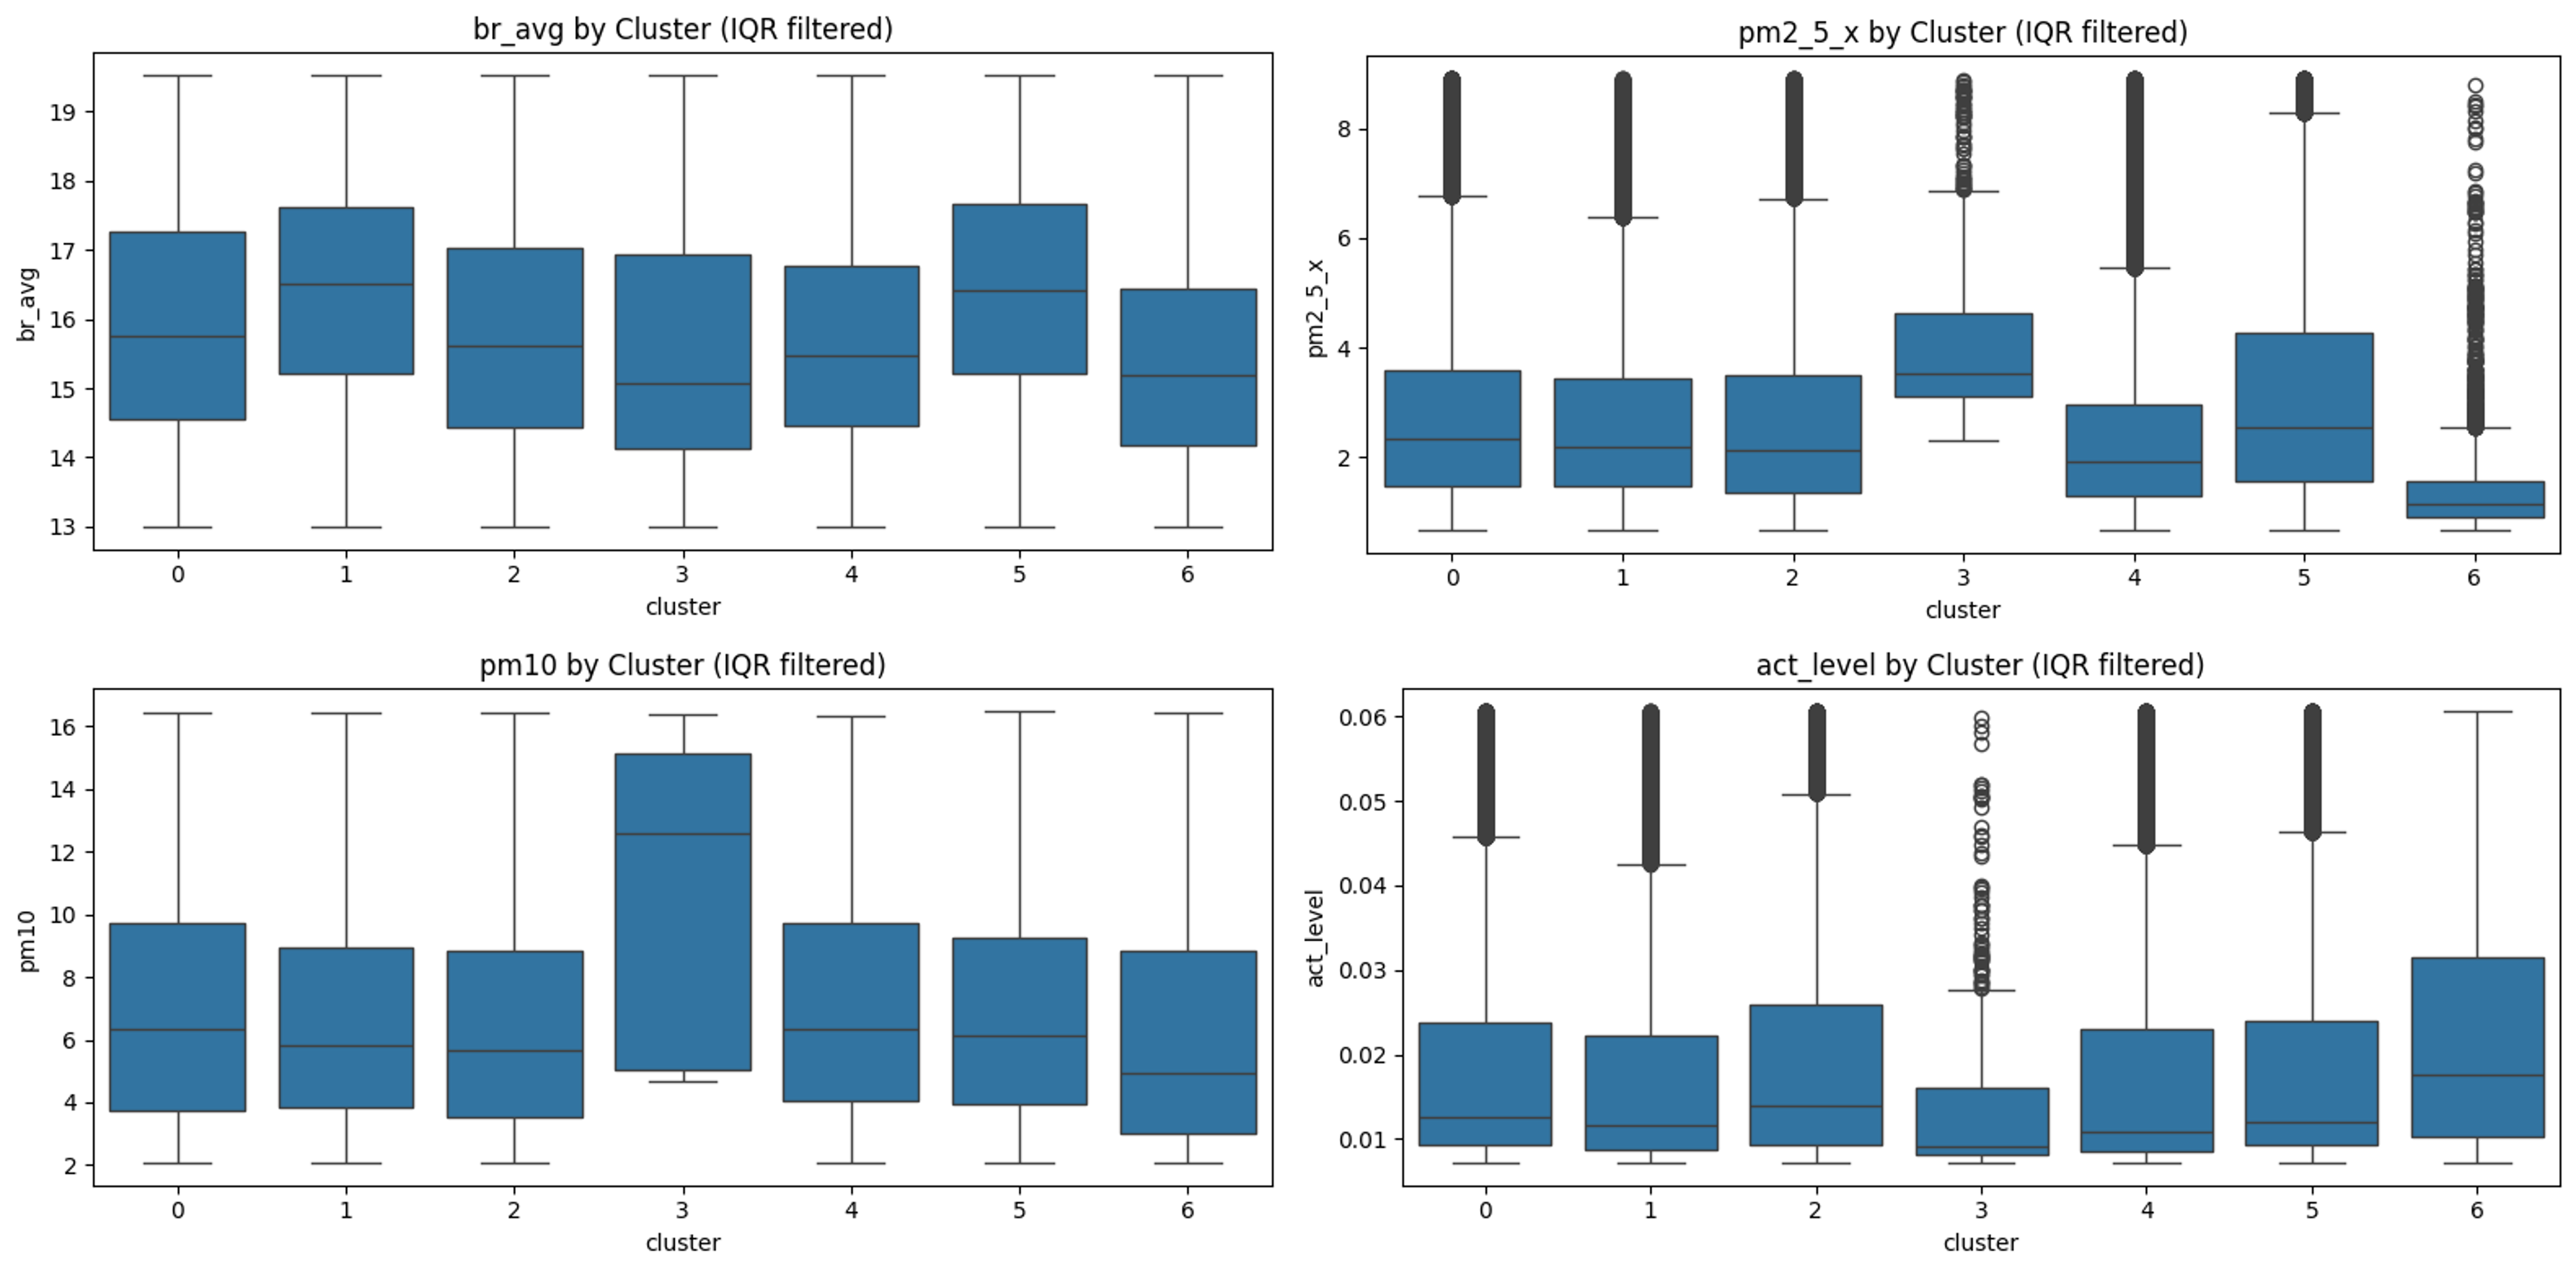
\includegraphics[width=6.44065in,height=1.85385in]{media/image6.emf}

Figure 5: \emph{Project timeline outlining key phases, including project
plan, data preprocessing, model development, and report writing, with
optional extension to clinical measures.}

The project is structured around four key phases, beginning with the
definition of the research objectives and an in-depth literature review,
as explained in figure 4. The subsequent phase involves the development
of a data preprocessing pipeline to align the datasets and identify the
most relevant features influencing physiological response.

Insights gained from both the literature and initial data analysis will
guide the design of the model architecture. A time-series
encoder-decoder transformer will be implemented to capture temporal
dependencies and learn latent representations that form an identity map
between pollution exposure and physiological response. These
representations will be used to predict future physiological states
under varying pollution conditions.

Several potential challenges have been identified that may impact the
timeline. First, missing or corrupted data may compromise model
reliability. As a mitigation strategy, any feature with more than 70\%
missing values will be excluded, as such sparsity limits the ability to
distinguish between true outliers and artefacts. Second, model
interpretability poses a notable limitation. To address this, SHAP will
be used to quantify the contribution of each input feature and improve
the transparency of the transformer model predictions (Lundberg \& Lee,
2017){[}9{]}.

If, after the training of the global model and subsequent fine-tuning at
the individual level, performance remains unsatisfactory, additional
clinical data will be integrated. These include lung function metrics,
cardiovascular inflammation markers, and stress-related indicators.
While these data may be temporally constrained, they offer additional
context that could enhance the model's predictive power.

The ultimate objective is to develop a robust and interpretable
framework capable of delivering personalised forecasts of physiological
responses to pollution exposure, contributing to both individual-level
health monitoring and broader public health strategies.

\hypertarget{references}{%
\section{6. References}\label{references}}

\begin{enumerate}
\def\labelenumi{\arabic{enumi}.}
\item
  World Health Organization Overview (2025) Available at:
  \url{https://www.who.int/health-topics/air-pollution\#tab=tab_1} (09
  June 2025).
\item
  Roos, L.G. and Slavich, G.M. (2023) `Wearable Technologies for health
  research: Opportunities, limitations, and practical and conceptual
  considerations', Brain, Behavior, and Immunity, 113, pp. 444--452.
  doi:10.1016/j.bbi.2023.08.008.
\item
  He, Q. and Ji, X. (James) (2021) `The labor productivity consequences
  of exposure to particulate matters: Evidence from a Chinese National
  Panel Survey', International Journal of Environmental Research and
  Public Health, 18(23), p. 12859. doi:10.3390/ijerph182312859.
\item
  Bernasconi, S., Angelucci, A. and Aliverti, A. (2022) `A scoping
  review on wearable devices for environmental monitoring and their
  application for Health and Wellness', Sensors, 22(16), p. 5994.
  doi:10.3390/s22165994.
\item
  Hu, K. et al. (2014) `Personalising pollution exposure estimates using
  wearable activity sensors', 2014 IEEE Ninth International Conference
  on Intelligent Sensors, Sensor Networks and Information Processing
  (ISSNIP), pp. 1--6. doi:10.1109/issnip.2014.6827617.
\item
  Verma, A., Ranga, V. and Vishwakarma, D.K. (2024) `Breath-net: A novel
  deep learning framework for no2 prediction using bi-directional
  encoder with Transformer', Environmental Monitoring and Assessment,
  196(4). doi:10.1007/s10661-024-12455-y.
\item
  Atzeni, M. et al. (2025) `A machine learning framework for short-term
  prediction of chronic obstructive pulmonary disease exacerbations
  using personal air quality monitors and lifestyle data', Scientific
  Reports, 15(1). doi:10.1038/s41598-024-85089-2.
\item
  Li, Y. et al. (2020) `Behrt: Transformer for Electronic Health
  Records', Scientific Reports, 10(1). doi:10.1038/s41598-020-62922-y.
\item
  Scott M. Lundberg and Su-In Lee. 2017. A Unified Approach to
  Interpreting Model Predictions (NeurIPS'17). In Neural Information
  Processing Systems (NeurIPS'17), 17212--17223.
\item
  Vaswani, A., Shazeer, N., Parmar, N., Uszkoreit, J., Jones, L., Gomez,
  A.N., Kaiser, Ł. \& Polosukhin, I., 2017. Attention is all you need.
  In Advances in Neural Information Processing Systems (NIPS 2017).
\end{enumerate}

\end{document}
